Das Hauptziel der Anwendung vieler Methoden des Machine Learning ist es, gute Vorhersagen zu treffen, im Gegensatz zur statistischen und bayesianischen Inferenz, die versucht, die zugrunde liegenden Mechanismen und Unsicherheiten in den Daten zu verstehen. \cite{lovelace2019}
``Geocomputation with R'' führt diese Methoden zur Anwendung statistischen Lernens und Mustererkennung in georeferenzierten Daten anhand von Fallstudien zu landslide susceptibility eines Areals in Südequador bzw. der Modellierung des floristischen Gradienten in Nebeloasen Südamerikas an, Ziel dieser Arbeit war es, diese Verfahren miteinander zu vergleichen und die allgemeine Methodik zum Import und Prozessieren georeferenzierter Daten in R anzuwenden und zu vertiefen. Nicht nur wurden predictive Maps für die Habitateignung Bayerns für Menschen aus der Eisenzeit erstellt, auch wurde ein Problem bei der Wahl eines optimalen Bufferradius zum Sampling von Punkten aus dem Studiengebiet diskutiert und mit einer interaktiven Shiny \cite{shiny} Applikation verdeutlicht und visualisiert. Abgesehen davon konnte auch mittels drei verschiedener Verfahren zur Berechnung minimaler Distanzen zu Gewässern gezeigt werden wie flexibel und effizient R für Geoprocessing sein kann. Abschließend sollten herkömmliche Cross Validation und spatial Cross Validation zur Bewertung der prädiktiven Performance aller Modelle gegenübergestellt und die Vor- und Nachteile beider Ansätze diskutiert werden. 

\begin{figure}[H]
    \centering
    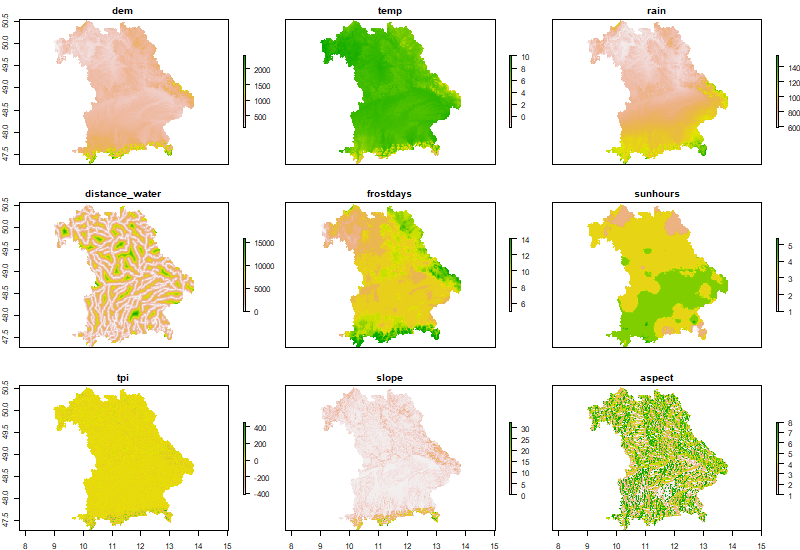
\includegraphics[width = 15cm, height = 12.5cm]{Figures/predictorstack.png}
    \caption{Plots der Variablen die für die Konstruktion des Datensatzes verwendet wurden. Zugang und Aufbereitung der Daten werden in Kapitel 2 behandelt.}
    \label{predictorstack}
\end{figure}